\newcommand{\sheet}{3}
\documentclass{article}
\usepackage[english, german]{babel}
\usepackage{amsthm,amssymb,amsmath,mathrsfs,mathtools}
\usepackage[shortlabels]{enumitem}
\usepackage{hyperref}
\usepackage{biblatex}
\usepackage{tikz}
\usepackage{tikz-cd}

% \usepackage[tmargin=1.25in,bmargin=1.25in,lmargin=1.2in,rmargin=1.2in]{geometry}


\newcommand{\C}{\mathbb{C}}
\newcommand{\R}{\mathbb{R}}
\newcommand{\N}{\mathbb{N}}
\newcommand{\Q}{\mathbb{Q}}
\newcommand{\Z}{\mathbb{Z}}
\newcommand{\Proj}{\mathbb{P}}
\newcommand{\Aff}{\mathbb{A}}

\DeclareMathOperator{\id}{id}
\DeclareMathOperator{\im}{im}
\DeclareMathOperator{\GL}{GL}
\DeclareMathOperator{\sgn}{sgn}
\DeclareMathOperator{\Tor}{Tor}
\DeclareMathOperator{\Sym}{Sym}
\DeclareMathOperator{\coker}{coker}
\DeclareMathOperator{\Quot}{Quot}
\DeclareMathOperator{\supp}{supp}
\DeclareMathOperator{\Hom}{Hom}
\DeclareMathOperator{\Spec}{Spec}
\DeclareMathOperator{\MinSpec}{MinSpec}
\DeclareMathOperator{\MaxSpec}{MaxSpec}
\DeclareMathOperator{\diag}{diag}
\DeclareMathOperator{\BL}{BL}
\DeclareMathOperator{\Ouv}{Ouv}
\DeclareMathOperator{\Sh}{Sh}
\DeclareMathOperator{\PSh}{PSh}
\DeclareMathOperator{\Eq}{Eq}
\DeclareMathOperator{\colim}{colim}
\DeclareMathOperator{\Pic}{Pic}
\DeclareMathOperator{\CL}{CL}
\DeclareMathOperator{\eq}{eq}
\DeclareMathOperator{\codim}{codim}

\newenvironment{exercise}[1] {
  \vspace{0.5cm}
  \noindent \textbf{Exercise~{#1}.}
} {
  \vspace{0.5cm}
}
\newenvironment{claim} {
  \par\noindent\textbf{Claim.}
} { }

\newenvironment{proof_claim} {
  \par\noindent\textbf{Proof of claim.}
} {
    \qed (of claim)
}

\title{Algebraic geometry 1\\Exercise sheet \sheet}
\author{Solutions by: Eric Rudolph and David Čadež}

\date{\today}


\begin{document}

\maketitle{}

Hey, sorry for submitting so weirdly, we usually submit to Robin, but this week
I remembered a few minutes after midnight and the field for submittion was already
closed in his group, and here it was still open. I also couldn't find his email
immediately to send him the sheet. Could you please forward him this pdf, please :)
Thank you

\begin{exercise}{1}
    We know that dominant morphisms between integral schemes map generic point
    to the generic point. So we get inclusion $k(\eta_X) \hookrightarrow
    k(\eta_Y)$.

    Integral schemes are irreducible, so any non-empty open subset is dense. Therefore we
    can focus on some affine neighbourhood of $X = \Spec(A) \subset X$, which we
    also name $X$. Then take preimage and 
    \dots
\end{exercise}

\begin{exercise}{2}
    \begin{enumerate}[label=(\roman*)]
        \item{
                Observe that for every $x \in X$ we have
                \begin{equation*}
                    \dim_{k(x)} H_i(C_\bullet \otimes_A k(x)) = \dim_{k(x)} \ker
                    (d_i \otimes k(x)) - \dim_{k(x)} \im (d_{i+1} \otimes k(x))
                \end{equation*}
                A map of finite free $A$-modules can be represented by a matrix
                with values in $A$.

                Let $M$ be an $m \times n$ matrix representing a map $A^n \to
                A^m$. Localizing at $x \in X$, we get a map
                \begin{equation*}
                    k(x)^n \cong A^n \otimes_A k(x) \to A^m \otimes_A k(x) \cong
                    k(x)^m
                \end{equation*}
                given by this ``same'' matrix, denoted by $M_x$, whose
                components are images of components in $M$ under $A \to k(x)$.
                
                Suppose now $M$ has rank $r$ at some point $x \in X$.
                Therefore there exists an invertible minor of size $r
                \times r$, call it $N$. That means that $\det N$ does not vanish in $x$.
                Then $D(\det N)$ is an open neighbourhood of $x$ on which $M$ has rank $\geq r$.

                This shows that $x \mapsto \dim_{k(x)} \im(M \otimes k(x))$ is
                lower semicontinuous.

                Multiplying function with $-1$ will switch upper and lower
                semicontinuity.

                Also note that for a given matrix we have $n = \dim \ker + \dim
                \im$ for every $x$ where $n$ is the dimension of the source.

                Considering all that we obtain that
                \begin{equation*}
                    x \mapsto \dim_{k(x)} \ker (d_i \otimes k(x)) - \dim_{k(x)} \im
                    (d_{i+1} \otimes k(x))
                \end{equation*}
                is a sum of upper semicontinuous function, so itself upper semicontinuous.
            }

        \item{
                We have $\beta^{-1}_i(n) = \beta^{-1}_i((-\infty, n + 1)) \cap
                \beta^{-1}_i([n, \infty))$, so intersection of an open and
                closed set, in particular it is constructible.
            }
        \item{
                Let $k = \bar{k}$ be a field and
                \begin{equation*}
                    C_\bullet \colon \dots \to 0 \to k[t] \to k[t] \to 0 \to \dots
                \end{equation*}
                be the complex of $k[t]$-modules, where the only nontrivial map
                is $1 \mapsto t$.
                We take homology at $k[t] \to k[t] \to 0$.
                We claim that it is not locally constant at closed point $(t) \in
                \Aff^1_k$.

                Take $x = (t - a)$ for $a \in k$, then
                \begin{equation*}
                    C_\bullet \otimes_{k[t]} k(x) \colon \dots \to 0 \to k \to k
                    \to 0
                \end{equation*}
                where the unique nontrivial map is $1 \mapsto a$.
                Clearly the image of $k \to k$ will be a $1$-dimensional $k$-vsp
                for $a \not= 0$ and $0$-dimensional for $a = 0$.

                For $x = (0)$ the generic point, we get a surjection $k(t) \to k(t), 1
                \mapsto t$.

                So
                \begin{equation*}
                    \dim_{k(x)} H(C_\bullet \otimes_{k[t]} k(x)) =
                    \begin{cases}
                        1 & x = (t) \\
                        0 & x = (t-a)\ \text{for}\ a \not= 0\ \text{or}\ x = (0)
                    \end{cases}
                \end{equation*}
            }
    \end{enumerate}
\end{exercise}

\begin{exercise}{3}
    \begin{enumerate}
        \item
            We have
            \begin{equation*}
                \begin{split}
                    X &= \Spec(A) \\
                    &= \Spec(R[T, T_1, T_2] / I_1 \cap I_2) \\
                    &= \Spec(R[T, T_1, T_2] / I_1) \cup \Spec(R[T, T_1, T_2] / I_2)
                \end{split}
            \end{equation*}
            where
            \begin{equation*}
                \begin{split}
                    X_1 = \Spec(R[T, T_1, T_2] / I_1) &= \Spec(R[\pi^{-1}, T_1, T_2]) \\
                    &= \Spec(R[\pi^{-1}][T_1, T_2]) \\
                    &= \Spec(K[T_1, T_2]) \\
                    &= \Aff^2_K
                \end{split}
            \end{equation*}
            and
            \begin{equation*}
                \begin{split}
                    X_2 = \Spec(R[T, T_1, T_2] / I_2) &= \Spec(R[T]) \\
                    &= \Aff^1_R.
                \end{split}
            \end{equation*}
            To show that $X$ is equidimensional, we have to check that both irreducible
            components have dimension $2$.
            Clearly they both do;
            $X_1$ is an affine plane over a field, and from Alg 1 we know $\dim \Aff^1_R
            = \dim R + 1 = 2$ since $R$ is a PID that is not a field.
        \item
            Clearly only prime ideal that contains $I_1 \cup I_2$ is $(\pi T - 1, T_1,
            T_2)$ which is consequently also a closed point.
            Denote $x = (\pi T - 1, T_1, T_2)$.

            To calculate $\dim \mathcal{O}_{X_1, x}$ we have to find ideals that
            are between $I_1$ and $x$. Those are exactly primes of
            $K[T_1, T_2]_{(T_1, T_2)}$, so $\dim \mathcal{O}_{X_1, x} = 2$.

            And for $\dim \mathcal{O}_{X_2, x}$ we have to find ideals that are
            between $I_2$ and $x$. Those are prime ideals of $R[T]_{(\pi T -
            1)}$. This is same as asking what is the height of $(\pi T - 1)$,
            which is $1$, so the localization has dimension $1$.
    \end{enumerate}
\end{exercise}

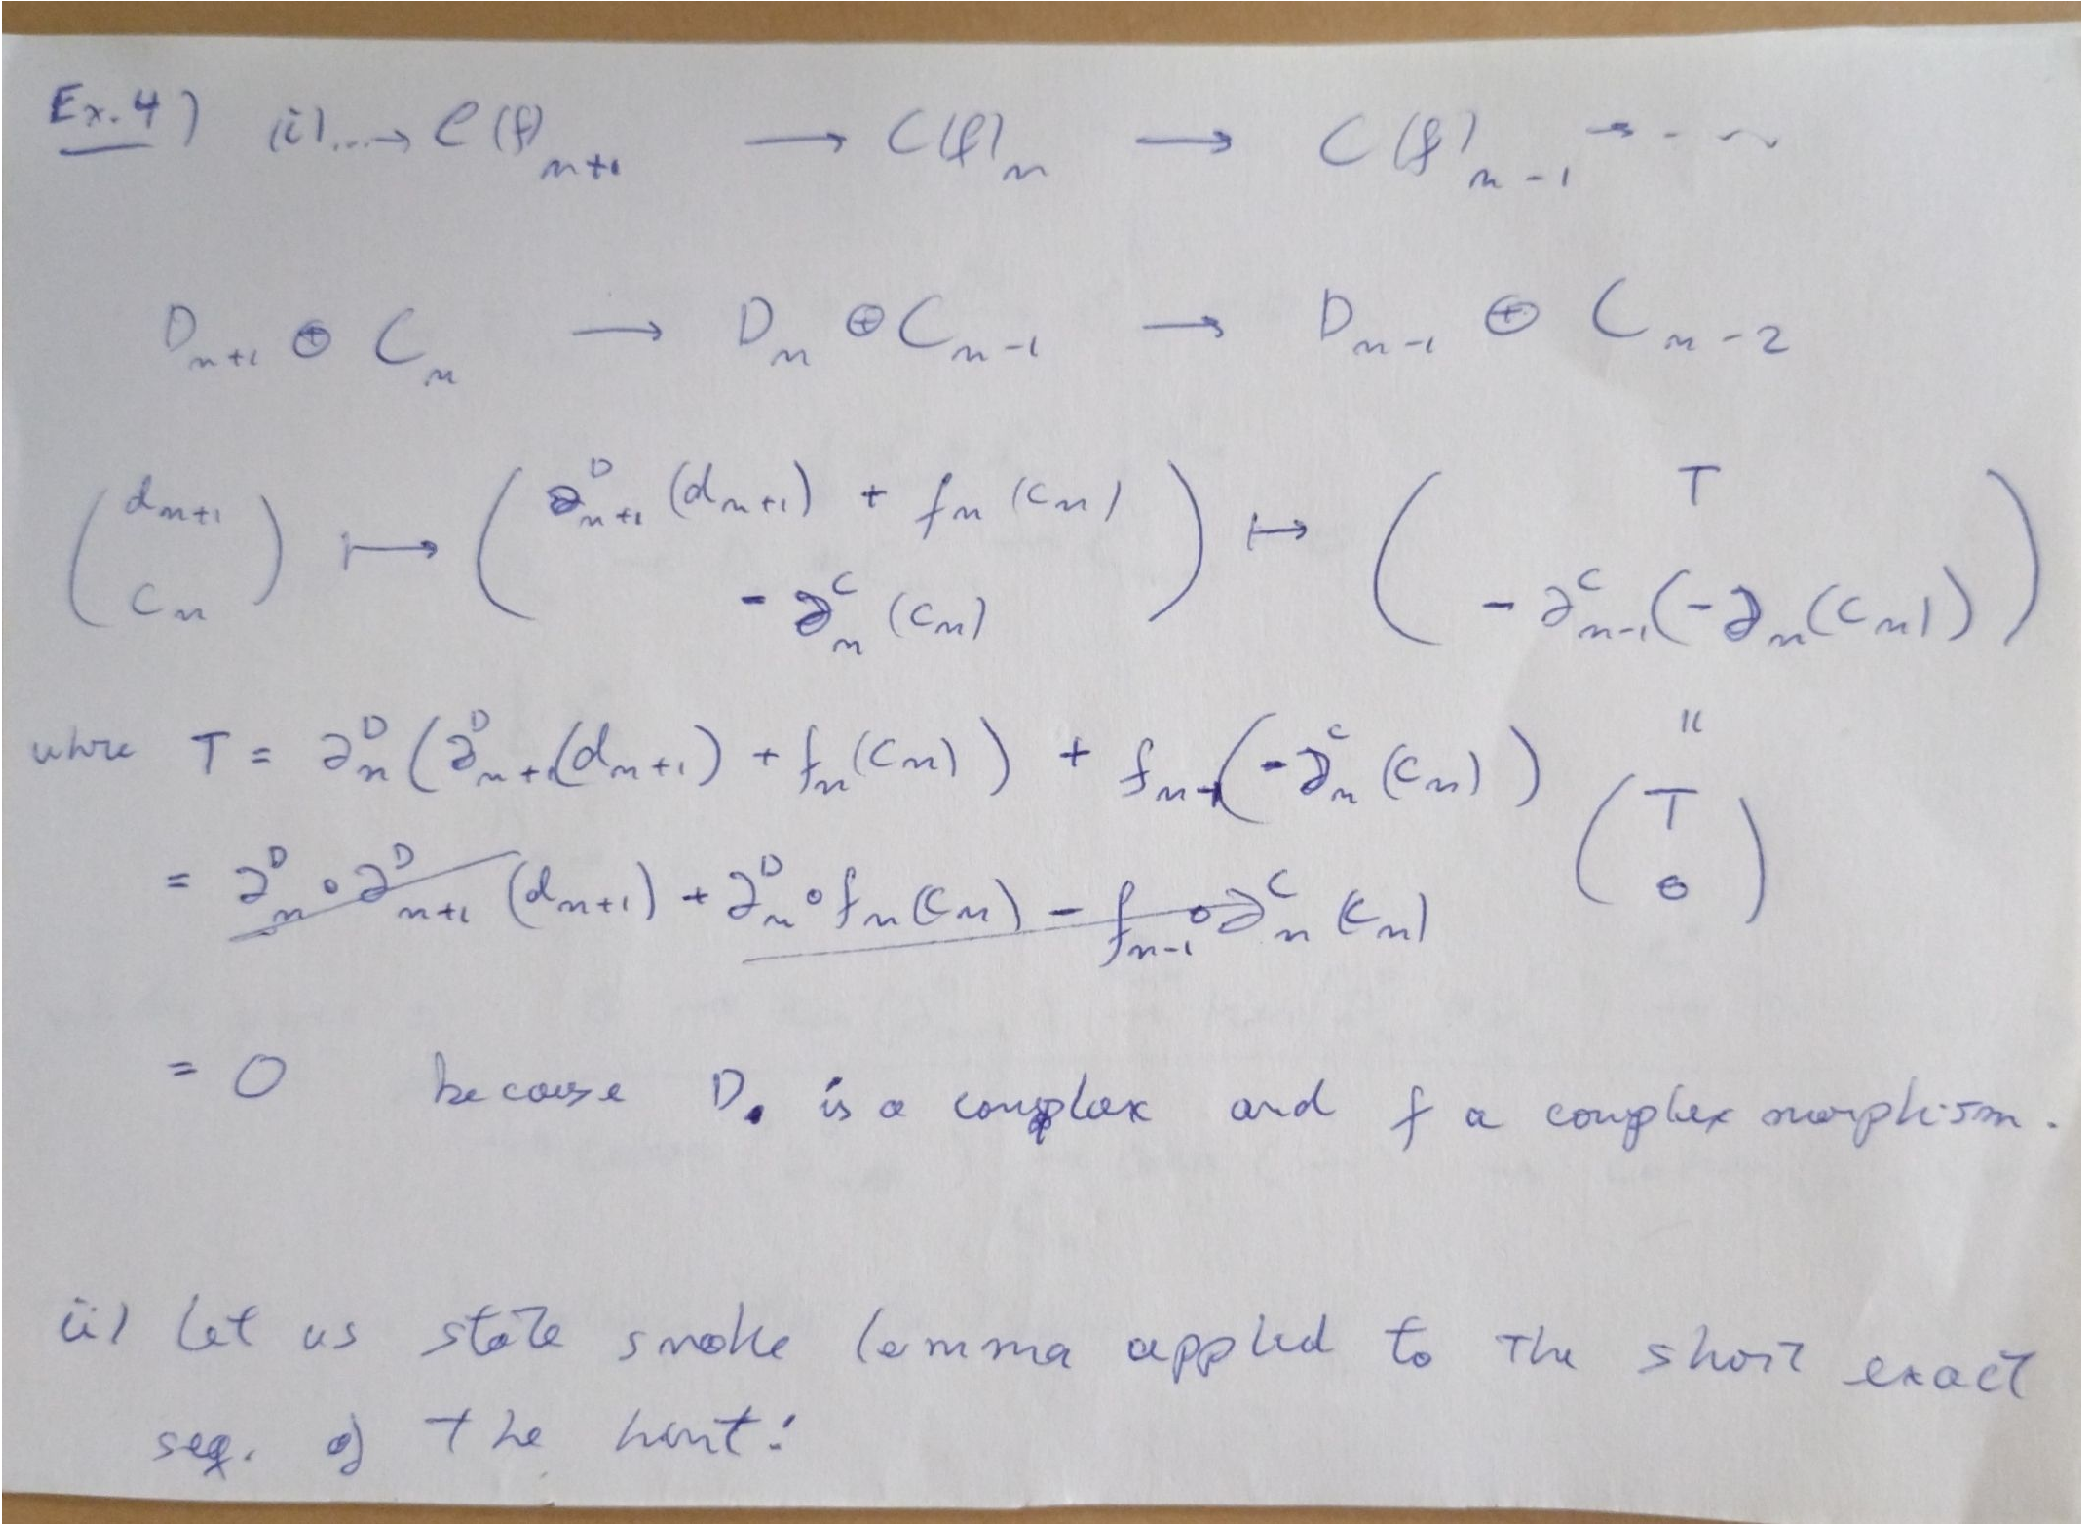
\includepdf[pages=-]{sheet3-exercise4.pdf}

\end{document}
